%!TEX root = thesis.tex

% ~10 pages 

\chapter{Design}
\label{chap:design}

This thesis aims to design a method that uses the semantic web to improve sensor data discovery as well as the integration and aggregation of sensor data from multiple sources. The outline of this method will be described in this chapter using the existing methods from Chapter \ref{chap:methods}. 

\section{Creating linked data from sensor metadata}

The process of automatically creating linked data from sensor metadata is shown in Figure \ref{fig:WPS1}. A \ac{wps} contain processes for retrieving metadata, converting it to linked data and outputting it to a triple store. Data from a \ac{sos} is retrieved by a \ac{wps} process. This process converts it to linked data. The output is an \ac{rdf} document containing the metadata as triples. These documents are posted to a \ac{sparql} endpoint, where they can be queried.  

The workflow of this \ac{wps} process is shown in Figure \ref{fig:WPS1workflow}. It is an adaption of the workflow by \cite{LD:Missier}, which was originally intended for creating linked data about vector parcel data. The input of the process should be the \ac{http} address of a \ac{sos}. Since both the requests and the data model are standardized in a \ac{sos} the process should be able to automatically perform the tasks for creating linked data. The first step is to make requests to the \ac{sos} to retrieve it's metadata. This results in a number of \ac{xml} documents that need to be filtered. The second step is to map the data inside these \ac{xml} documents to linked data ontologies. In the final step \ac{rdf} documents are created of the mapped metadata and published on the web.  

\begin{figure}
	\centering
	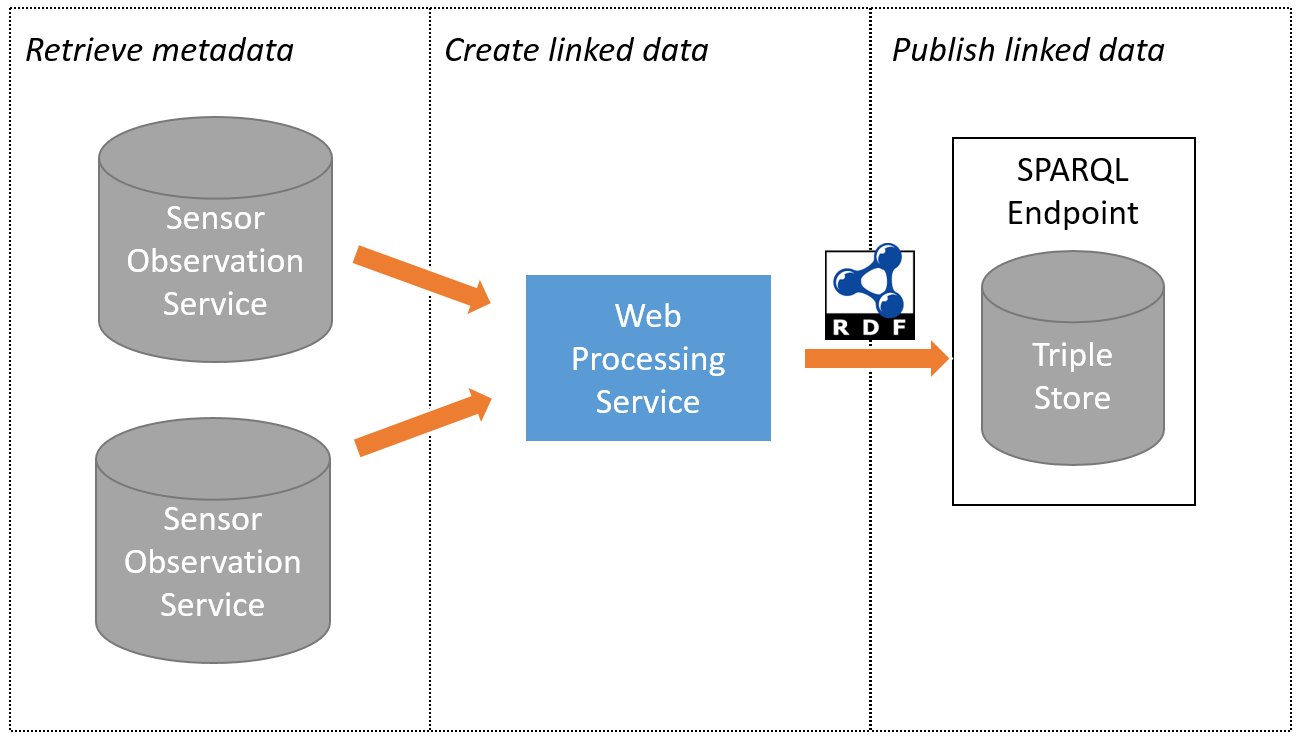
\includegraphics[width=0.8\linewidth]{UML/wps1diagram.PNG}
	\caption{General overview of creating linked data of metadata from Sensor Observation Services}
	\label{fig:WPS1}
\end{figure}

\begin{figure}
	\centering
	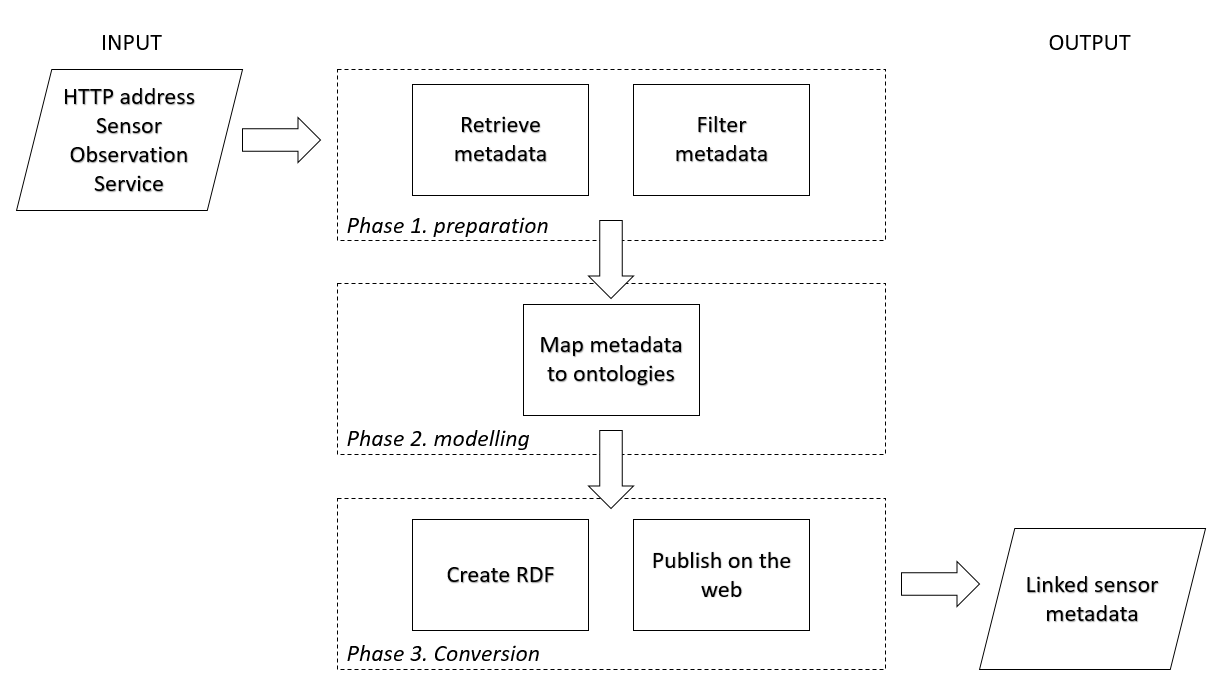
\includegraphics[width=1\linewidth]{UML/wps1workflow.PNG}
	\caption{Workflow diagram of Web Processing Service (adapted from \cite{LD:Missier})}
	\label{fig:WPS1workflow}
\end{figure}

\subsection{Retrieving metadata from the Sensor Observation Service}
\label{chap:retrieveSOS}

The first step of creating an online knowledge base with sensor metadata is to retrieve the metadata from the different \aclp{sos}. This data has to be understood in order to map it to an ontology and it should be filtered to only contain the required parts of data. The next paragraphs will describe the way sensor metadata is modelled in a \ac{sos}, with which requests it can be retrieved and how it should be filtered. 

\subsubsection{Sensor metadata model}
A sensor observation service describes a number of its properties that are required to know in order for clients to request data from it. It identifies the organisation that maintains it, with at least the organisation's name and its contact information. Optionally, the organisations website, keywords and an abstract about the \ac{sos} can be supplied. The \ac{sos} also describes its identifier and \ac{http} addresses (the address for sending requests can differ for POST or GET requests). It also lists the \ac{sos} versions and response formats it supports. The access constraints and fees are also mentioned. In most cases the use is free of charge and without access constraints. However, it is possible for an organisation to restrict the use of the \ac{sos} in these ways.  

In the \ac{swe} standards a sensor is modelled using two entities: a procedure and a \acf{foi}. The procedure is the method of sensing and the \ac{foi} is the feature of which the sensor is sensing a certain property. Therefore, the observable property ties together the procedure and feature of interest. It should be noted that the geometry of a \ac{foi} is not necessarily always a point geometry. It can also be generalized into larger features (e.g. multiple sensors observing different parts of one lake). 

In version 2.0 of the \acl{sos} Interface Standard \citep{SW:OGC2} an offering is defined as a grouping of \acp{foi}, which have a common procedure. The constraint of sharing the same procedure has been added in version 2 of this document to solve the ambiguity of offerings in \ac{sos} 1.0. The purpose of offerings is to allow users to query the observation data more efficiently. \acp{foi} that are often queried together are therefore grouped into the same offering for efficient retrieval.        

\begin{figure}
	\centering
	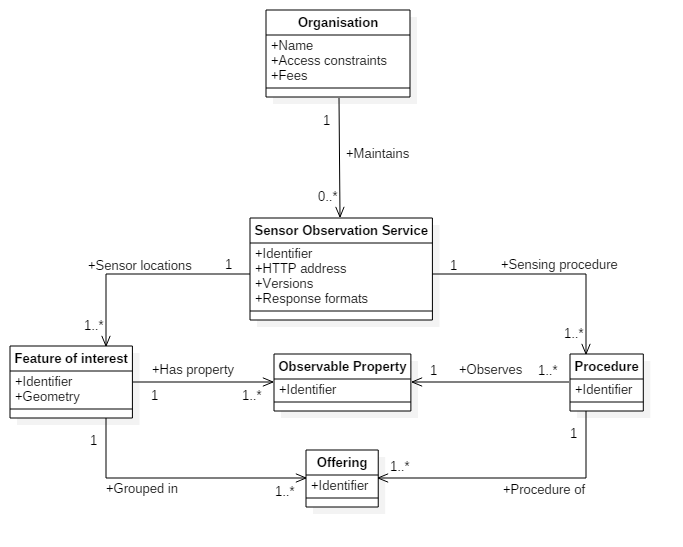
\includegraphics[width=\linewidth]{UML/SOS_UML.PNG}
	\caption{Sensor metadata derived from a \ac{sos}}
	\label{fig:SOS_UML}
\end{figure}

\subsubsection{Metadata Requests}
\label{par:metadataRequests}
To retrieve metadata from a \ac{sos} a \texttt{GetObservation} request is made first. This is a request with a very generic structure. The GET request is created by adding \url{service=SOS\&request=GetCapabilities} to the \ac{http} address of the \ac{sos}. For example, the \ac{rivm} has its \ac{sos} at the address: \url{http://inspire.rivm.nl/sos/eaq/service?}. Therefore, the capabilities document can be retrieved using the following \ac{url}: \url{http://inspire.rivm.nl/sos/eaq/service?service=SOS&request=GetCapabilities}. 

This requests returns the capabilities document of the \ac{sos} (see Paragraph \ref{par:capabilities}). This lists the identifier of each \ac{foi}, each procedure and each observed property. It also has a section where the offerings that it contains are being described. This description of an offering includes a unique identifier, a procedure and the corresponding observed property. Additionally, descriptions can be added such as a bounding box, temporal range, \ac{foi} type and response format.  

\begin{sloppypar}
	Unfortunately, the capabilities document is not able to provide information about which procedure is being applied for which feature of interest. This is crucial information for knowing which deployed sensors can be queried using a particular \ac{sos}. Also, the features' geometries cannot be retrieved from the capabilities document. Based on that document it is not yet clear which sensor locations are being used and what is measured at a specific location. Therefore, a \texttt{GetFeatureOfInterest} request can be made to retrieve the location of each \ac{foi}. Such a request can be made by adding \url{service=SOS&version=2.0.0&request=GetFeatureOfInterest}. The version \ac{kvp} should correspond to the version declared in the capabilities document. A pointer to a specific \ac{foi} is optional and usually all \acp{foi} are returned by default. Using the example of the \ac{sos} by the \ac{rivm} the \texttt{GetFeatureOfInterest} request looks like this: \url{http://inspire.rivm.nl/sos/eaq/service?service=SOS&version=2.0.0&request=GetFeatureOfInterest}.    
\end{sloppypar}

On the one hand, a \texttt{GetFeatureOfInterest} document does not necessarily provide information about the procedures that are related to a certain feature of interest. On the other hand, a \texttt{DescribeSensor} request does not always relate the process to a \ac{foi} either. However, a \texttt{GetObservation} requests return observation data grouped per feature of interest. Therefore, small amounts of data can be retrieved from each offering using \texttt{GetObservation} requests to link the \acp{foi} to procedures and observed properties. When possible a temporal filter should be used to limit the data traffic. Using this method every procedure and offering can be related to a set of \acp{foi} with their corresponding geometry. This represents the collection of sensor devices of which data can be retrieved by sending requests to the \ac{sos}. 

\subsubsection{Filter Metadata}

The documents that are returned by the \ac{sos} contain a lot of information. In some cases the returned information can be limited by adding filters to the requests. However, not all \ac{sos} have supported all filters and not all unnecessary data can be filtered out. Therefore, the \ac{xml} documents that are returned should often be filtered on the client side. In a \ac{xml} document every element should be defined using a namespace. Often these prefixes are defined in the xmlns tag at the top of the document to refer to these namespaces. These namespaces and corresponding tags can be used to filter the response documents for the content that is required. It should be noted that there are multiple namespaces that could be used to define the same concept. However, the potential namespaces that can be encountered are restricted by the schema describing the content of a response document. This schema is usually referenced to in the start tag of the response document.


\subsection{Modelling with the om-lite and sam-lite ontologies}
\begin{figure}
	\centering
	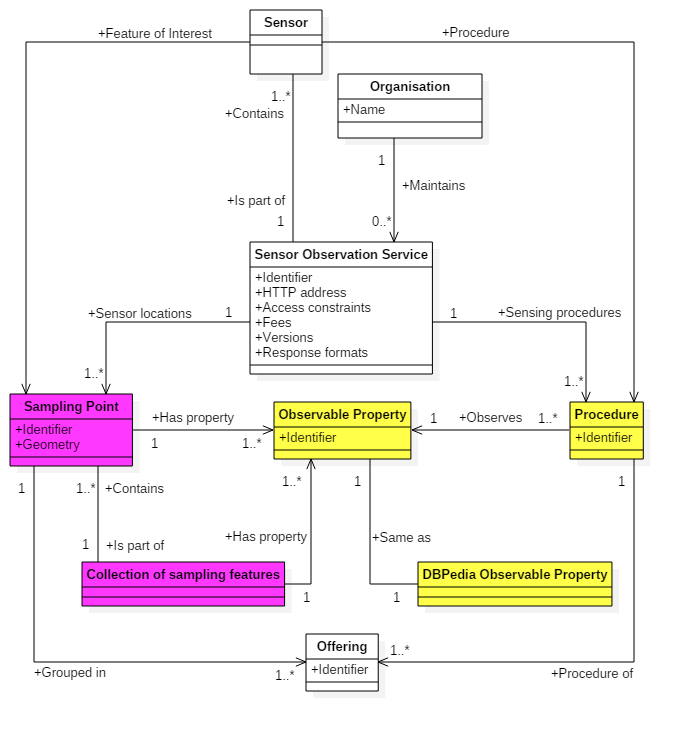
\includegraphics[width=1\linewidth]{UML/SOS_Semantic_UML_2.PNG}
	\caption{Sensor metadata as modelled in RDF (om-lite classes in yellow and sam-lite classes in purple)}
	\label{fig:SOS_Semantic_UML}
\end{figure}

After the metadata has been retrieved from the \ac{sos} and filtered (Figure \ref{fig:SOS_UML}) it has to be mapped to linked data ontologies. For this the om-lite and sam-lite ontologies are being used in combination with the PROV and GeoSPARQL ontologies. Figure \ref{fig:SOS_Semantic_UML} shows the which ontologies that can be used to describe the classes of Figure \ref{fig:SOS_UML}.   

A \ac{sos} is modelled as an agent with a specific name, that acts on behalf of a certain organisation. The organisation, access constraints, fees, versions and response formats are properties of the \ac{sos}. Every sensor is described by a procedure and a certain feature of interest. The sensor class was not present in the model of Figure \ref{fig:SOS_UML}, because the \ac{sos} does not define sensors. However, the sensor class has been added to the semantic model to make the relation between procedure and sampling point explicit. 

In Figure \ref{fig:SOS_Semantic_UML} the collection of sampling features is added. These are collections of all \acp{foi} from different \aclp{sos} of which the same property is being observed. The sampling collections are currently modelled to only contain sampling points. This is because the \ac{foi} of an air quality sensor is equal to the bubble of air directly around the sampling point. Other types of sampling features can be added when the application requires this. The offering class is modelled as a specialization of the collection of sampling features. It contains a subset of the sampling points that are part of the same offering at a particular \ac{sos}.

The last class that has been added to the model as shown in Figure \ref{fig:SOS_Semantic_UML} with respect to the model from Figure \ref{fig:SOS_UML} is the DBPedia observed property class. Every observed property that is defined in a \ac{sos} relates to a certain observed property as defined by DBPedia. Since \ac{sos} requests require their own identifiers as input the observed property class exists twice in the model: one as defined by the \ac{sos} and one as defined by DBPedia. For the same reason all sampling points, processes and offerings have a `name' attribute in addition to their \ac{uri}. These store the original (non-semantic) identifier that they were given by the \ac{sos}. 

\subsection{Output linked sensor metadata}
\label{par:publishLD}

Once the data has been retrieved and mapped to their corresponding classes in the ontologies \ac{rdf} triples can be created to link the data together. These triples should be stored in files and posted to a \ac{sparql} endpoint. The following two paragraphs will describe these steps in more detail.


\subsubsection{Create RDF}
\label{par:createRDF}
For every mapped part of metadata from the \ac{sos} one or more triples are created. These triples consist of at least of \acp{uri}. However, preferably they are \acp{url} that can be resolved to an \ac{rdf} document that contains semantic information about what it represents. To do so every part of metadata is automatically assigned a \acf{purl}. For this kind of \ac{url} to resolve a \ac{purl} server should be set up. This server performs one of the six tasks shown in Table \ref{tbl:HTTP} whenever a \ac{purl} is being retrieved. The structure of a \ac{purl} consists of the \ac{http} address of the \ac{purl} server, with a unique identifier attached to it. For example, \url{http://www.examplePURLServer.com/unique\_identifier}. 

Once the metadata is assigned \acp{purl} the triples can be created. Since the metadata of the sensors is being returned by the \ac{sos} in a structured way links can be created between \acp{url} of \acp{foi}, observable properties, procedures and the other classes shown in Figure \ref{fig:SOS_Semantic_UML}. After these triples have been created the linked data should be serialized to an \ac{rdf} document. For this a specific notation has to be selected.  


\begin{table}[]
	\centering
	\caption{Types of PURLs \citep{LD:PURL}}
	\label{tbl:HTTP}
	\resizebox{\textwidth}{!}{%
		\begin{tabular}{lll}
			PURL Type & Meaning                                         & HTTP Shorthand     \\
			301       & Moved permanently to a target \ac{url}          & Moved Permanently  \\
			302       & Simple redirection to a target \ac{url}         & Found              \\
			303       & See other \acp{url} (use for Semantic Web resources) & See Other     \\
			307       & Temporary redirect to a target \ac{url}         & Temporary Redirect \\
			404       & Temporarily gone                                & Not Found          \\
			410       & Permanently gone                                & Gone              
		\end{tabular}
	}
\end{table}

\subsubsection{Publish RDF on the web}
To store the linked data created under the previous paragraph a \ac{sparql} endpoint has to be set up. This endpoint is connected to a triple store. This means that the \ac{rdf} documents containing linked data can be send to it using POST requests. After it has been stored in the triple store users can query the triples using the \ac{sparql} query language. 

Once the linked data is inside the triple store the \acp{purl} can be redirected to \ac{sparql} \texttt{Describe} queries. A describe query takes a \ac{uri} as input and returns all the triples that contain this \ac{uri} as either an subject, predicate or object. This means that all information that the endpoint has about a particular \ac{uri} is being returned. If the \ac{purl} server receives a request for a particular \ac{purl} it makes a \texttt{Describe} query to the endpoint and returns to the client all the linked data that it retrieved about this \ac{purl}.  


\section{Using logical queries to retrieve sensor data}
The second web process looks on the semantic web for sensors that observe a certain property in a specific area. It collects the data for these sensors at their corresponding \acl{sos}. When multiple data sources are found the data is integrated into a single dataset. The sensor data is temporally aggregated before it is returned to the user. Optionally, spatial aggregation can be performed as well.

\subsection{Discovering sensors}
\label{par:discover}
For discovering sensors there are a number of input parameters for the second process: An observed property, a set of names of spatial features, a temporal range and granularity. Additionally, a type of spatial aggregation can be added. The input data is inserted in a number of \ac{sparql} queries. First the geometry is retrieved for all features inside the input list of features. This is done using the name or identifier attribute of spatial features at the endpoint.  

Then a second \ac{sparql} query selects the sensors that are part of a collection that observe a certain property of the \acp{foi}. This query also contains a spatial filter with the retrieved geometries. This makes sure only sensors in the requested areas are returned. For all discovered sensors the corresponding \ac{sos} \ac{url}, observed property, offering and process identifiers are retrieved. These original \ac{sos} identifiers are required for creating \texttt{GetObservation} requests.  

\subsection{Retrieving sensor data}
\label{par:retrieve}
 The \ac{sparql} queries return a table with all necessary information per sensor on each row. The columns of this table are: sensor \ac{uri}, \ac{foi} geometry, \ac{foi} identifier, procedure identifier, observed property identifier, offering identifier, and the last column contains the \ac{url} of the \ac{sos}. The data that is returned by the \ac{sparql} queries described in Paragraph \ref{par:discover} correspond to the \texttt{GetObservation} input parameters as described in Paragraph \ref{par:sos}. This request is send out using all the values per row in the returned table of sensor metadata and is structured by taking the \ac{url} of the \ac{sos} and extending it with: 
 \begin{quote}
 	\url{service=SOS&version=2.0.0&request=GetObservation&procedure=the_procedure&offering=the_offering&observedproperty=the_observed_property&responseformat=http://www.opengis.net/om/2.0&featureOfInterest=the_feature_of_interest}. 
 \end{quote} 
 
 If the \ac{sos} supports temporal filters these should be added to only retrieve observation data from the temporal range that the user is interested in. To include a temporal filter the following parameters can be added to the above GET request:
\begin{quote}
	\url{&temporalFilter=om:resultTime,start_time/end_time}
\end{quote} 


\subsection{Integrating and aggregation sensor data}
The requests described in Paragraph \ref{par:retrieve} result in a \ac{xml} document with observation data for every sensor. In each document the observations have to be retrieved, with their corresponding result time, phenomenon time and \ac{uom}. All of these observation have to be stored in a uniform way in another file or file-like object. If the temporal filter was not supported by the \ac{sos} the observation should only be stored if it is inside the requested temporal range. Also the \ac{foi} geometry should be stored with the observation for data visualisation or spatial aggregation later on. This process repeats itself until the observations have been retrieved from all \ac{xml} documents and they are all stored in a single dataset.  

The next step is to temporally aggregate the observation data. For every sensor location the result time is compared to the temporal range and the value for temporal granularity. It should then be appended to a list that corresponds to a certain subset of the temporal range. After this temporal sorting has been performed all observation values in a list should be aggregated according to a user defined method. 

If a spatial aggregation method is part of the user's logical query then this is performed after the temporal aggregation. For each of the spatial features for which observation data has been retrieved a single list of aggregated data is produced. This list contains the observation value for each time interval (with a length equal to the temporal granularity) inside the temporal range. The spatial aggregation is performed in a similar fashion as the temporal aggregation. First all observation data is order in a list per time interval per spatial feature. After all observations have been ordered the required aggregation method is performed to produce a single value for each of the lists. 

Examples of aggregation methods that can be used for spatial or temporal aggregation are the average, median, minimum, maximum or sum. Which method is being used is dependent on the information need of a user. Therefore, these methods can be extended with more complex aggregation techniques as described by \citep{SW:Ganesan}. Also, as \cite{SSW:Stasch4} argue a `check' could be implemented to make sure users do not (accidentally) request a meaningless type of aggregation, such as the sum of temperature values over a certain area. 


\chapter{Prototype implementation}
\label{chap:impl}
The prototype implementation serves as a proof of concept. It takes the designed method from Chapter \ref{chap:design} and applies it using existing software tools and python libraries and modules. First, the implementation of the process for automatically creating linked sensor metadata will be described. After that the implementation of the process for retrieving sensor data using logical queries is described. The third part of this chapter describes how the two processes have been made available online. The final part shows the web application that has been created as an interface for the second web process.

\section{Creating linked data from sensor metadata}

The first step of the method described in Chapter \ref{chap:design} is to automatically harvest sensor metadata from a \ac{sos} using various requests. This data should then be mapped to ontologies and serialized to an \ac{rdf} document. The next paragraphs will describe how these steps have been implemented using the Python programming language.

\subsection{Making sensor metadata requests}
A Python class object is created for the \ac{sos} based on Figure \ref{fig:SOS_UML}. This class contains the different variables and has built in functions to automatically retrieve the metadata. When a SOSclass instance is created the \ac{url} of the \ac{sos} has to be entered as input value. The initialisation of the SOSclass instance creates empty variables are created for storing information about the \ac{sos}' organisation, supported \ac{sos} versions, response formats, features of interest, offerings, observable properties and procedures. 

After the initialisation is finished the method \texttt{SOSclass.request()} is automatically triggered. This function starts by sending a \texttt{GetCapabilities} request to the \ac{sos}. For making \ac{http} GET and POST requests the Requests library for Python is used (see \url{http://docs.python-requests.org}). Listing \ref{lst:Requests} shows how to create a \texttt{GetCapabilities} request with the \ac{http} GET function from this library.

\begin{sloppypar}
	Based on the content that is being retrieved from the capabilities request further requests are being made. First, the geometries of the \acp{foi} are collected using \texttt{GetFeatureOfInterest} requests. Similar to the \texttt{GetCapabilities} there are no specific parameters required except for: \url{service=SOS&version=2.0.0&request=GetFeatureOfInterest}. However, one of the \aclp{sos} used in this thesis had implemented their \texttt{GetFeatureOfInterest} request to always require a feature id parameter. Therefore, the following exception had to be built in case this error is returned: \url{service=SOS&version=2.0.0&request=GetFeatureOfInterest&featureOfInterest=allFeatures}.
\end{sloppypar}

\begin{sloppypar}
After the geometries of the \acp{foi} have been retrieved they should be linked to procedures and observable properties. As described in Paragraph \ref{par:metadataRequests} it is not mandatory to define these relations in the \texttt{GetCapabilities}, \texttt{GetFeaturesOfInterest} or \texttt{DescribeSensor} response documents. Therefore, small amounts of observation data are requested from the sensors using \texttt{GetObservation} requests.  
\end{sloppypar}

\begin{lstlisting}[caption={Creating a HTTP Get request using Python's Request library}, label={lst:Requests}]
import requests

sosURL = "http://example.com/SOS?"

# Create the GetCapabilities request string
GetCapabilities = "{0}service=SOS&request=GetCapabilities".format(sosURL)

# Send the request
r = requests.get(GetCapabilities)

# Print the response document
print r.content

\end{lstlisting}   


\subsection{Map metadata to ontologies}
After each request is send an \ac{xml} document is returned. To retrieve data from these \ac{xml} documents the LXML library for Python is used (see \url{http://lxml.de}). With this library the \ac{xml} document can be loaded into an Python object, which allows for easy \ac{xml} processing, such as looping through the elements and searching the whole document for elements with specific tags. Listing \ref{lst:LXML} shows a snippet of code that takes the response document retrieved from Listing \ref{lst:Requests} and that uses the LXML library to find all offerings presented in this document. All offerings are returned as a list and stored inside the variable `SOSclass.offerings'. With this principle all metadata from the \ac{sos} is retrieved from the \ac{xml} response documents and stored for further processing.    

\begin{lstlisting}[caption={Creating an Etree object from an XML response document using Python's LXML library}, label={lst:LXML}]
import lxml

# Store the retrieved document as an Etree object
tree = etree.fromstring(r.content)

# Retrieve the namespaces from the XML document
nsm = tree.nsmap

# Find all subsets of the XML document that are inside a `sos:ObservationOffering' element
SOSclass.offerings = tree.findall(".//sos:ObservationOffering", nsm)

\end{lstlisting}   

Once all the relevant metadata has been retrieved from the \ac{sos} and stored inside the class object it should be mapped to linked data ontologies. For the Python package RDFlib is used (see \url{https://rdflib.readthedocs.org/}).  RDFlib defines an \ac{rdf} graph to which triples can be added. Listing \ref{lst:rdflib} shows a snippet of code that defines an \ac{rdf} graph and adds all procedures of a \ac{sos} to it with the type `http://def.seegrid.csiro.au/ontology/om/om-lite\#process'.


\begin{lstlisting}[caption={Creating an RDF graph object with the Python package RDFlib}, label={lst:rdflib}]
import rdflib

# The domain of the PURL server
PURLZ = "http://localhost:8099/masterThesis_tudelft"

# Create the OM-lite namespace 
om_lite = rdflib.Namespace('http://def.seegrid.csiro.au/ontology/om/om-lite#')

# Initialize a graph object
g = Graph()

for i, procedure in enumerate(SOSclass.procedures):
	# Define a URIs for the procedures
	procedureURI = URIRef("{0}/{1}_PROC_{2}".format(PURLZ, SOSclass.organisation, i))
	
	# Add all procedures to the graph and define them as om-lite processes
	g.add( ( uriProcedure, RDF.type, om_lite.process) )

\end{lstlisting}  

\subsection{Publish linked data}
create and post purl batches

For creating \aclp{purl} the Purlz software (\url{http://www.purlz.org/}) has been used. All \acp{uri} that are created get a \ac{purl} assigned to it. The \ac{purl} resolves the \ac{uri} to a \texttt{DESCRIBE} query at the endpoint. This query is structured as a get request: \texttt{\seqsplit{http://localhost/strabon-endpoint-3.3.2-SNAPSHOT/Describe?submit=describe\&view=HTML\&handle=download\&format=turtle\&query=DESCRIBE < an\_URI >}}. The request has `\texttt{/Describe?submit=describe}' to call the script that deals with describe queries and to tell it that the request is also submitting this kind of query. The parameters `\texttt{view=HTML\&handle=download}' indicate that the endpoint's website is requested, but the returned data should be a download file instead of an HTML page. The parameter `\texttt{\&format=turtle}' sets the \ac{rdf} notation of the download file to Turtle and `\texttt{\&query=DESCRIBE <an\_URI>}' is the \ac{sparql} query that contains the \ac{uri} between brackets. 

Every \ac{uri} is written to an \ac{xml} file with the parameters: ID, \ac{purl} type, and target address. Optionally, information about the person or organisation maintaining the \ac{purl} can be added. The ID is the original \ac{uri} that is being resolved to the target address. The \ac{purl} type is set to 303, which means that it refers the client to the target address. Alternative types can be found in Table \ref{tbl:HTTP}. After all \acp{uri} have been added to the so called \ac{xml} `batch' file \citep{LD:PURL2}, the file can be posted to the Purlz server. \\



serialize RDF graph
post RDF file to endpoint


Setting up the Strabon (Figure \ref{fig:Strabon}), Apache Tomcat and Pubby software. 

\begin{figure}
	\centering
	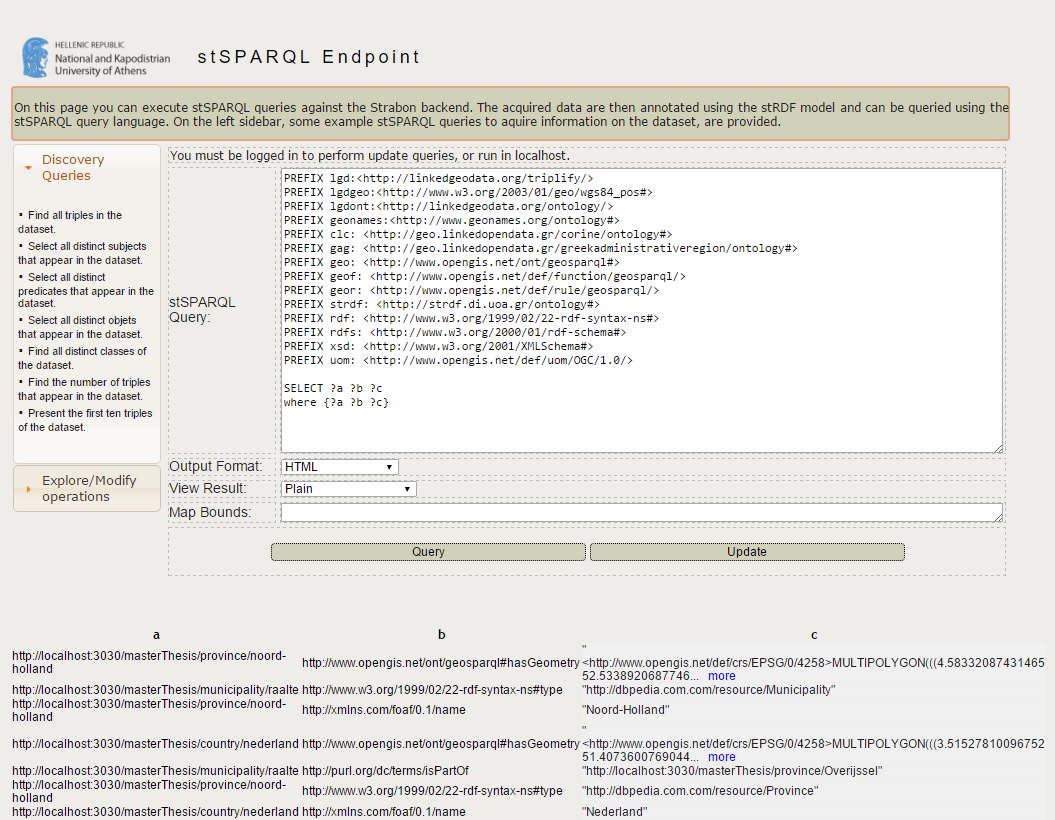
\includegraphics[width=\linewidth]{figs/Strabon.PNG}
	\caption{Strabon endpoint}
	\label{fig:Strabon}
\end{figure}

%\begin{figure}
%\centering
%	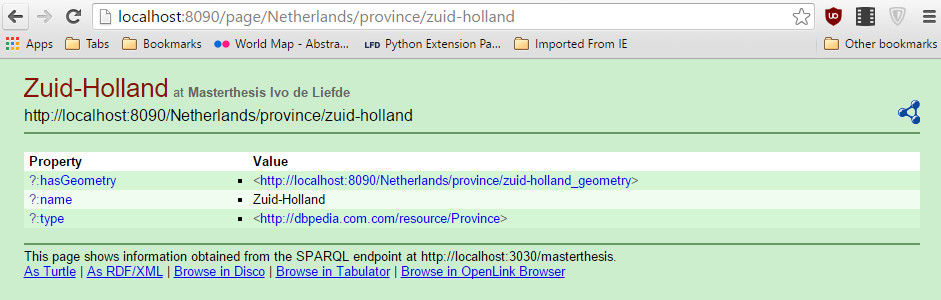
\includegraphics[width=\linewidth]{figs/pubby.PNG}
%	\caption{Pubby interface for \ac{rdf}}
%	\label{fig:Pubby}
%\end{figure}

The Strabon and Parliament endpoint have been tested since they both handle GeoSPARQL queries. Strabon has been used in the final design, because the Parliament endpoint rejected certain longer queries (see \ref{par:spQueries}).

Pubby software in combination with Apache Tomcat allows for a user interface that is easier to navigate through for humans. The links stored in \ac{rdf} triples are represented as hyperlinks which can be used to navigate between pages about different concepts. 



\section{Using logical queries to retrieve sensor data}

Explain how the second WPS is made 

\subsection{Input parameters}
The prototype takes a number of input parameters. First of all, a list with observed properties which will be the 'layers' that the process returns. The second parameter is the category of input features. This can be set to administrative units (country, province or municipality), land cover or raster. The third parameter is a list of input feature. This is a list of names or identifiers that correspond to the category. The next parameter is the temporal range. This has to be a list of two \ac{iso} datetime strings representing the start and end time. The fifth parameter is the temporal granularity, represented by an \ac{iso} delta datetime string. The sixth input parameter is the method of spatial aggregation. This method will be applied to aggregate the data based on the input features. The last input parameter is the temporal aggregation method to aggregate data between start and end time to the required granularity.      
% for the \ac{eea} reference grid.  

\subsection{Retrieving geometries}
The input category is a starting point for the process to find the geometries of the input features. It creates a \ac{sparql} query to retrieve the geometries of these features. 

\subsection{Spatial queries}
With the found geometries a \ac{sparql} query is made to find a sensor collection that has a certain observed property. From this collection sensors can be selected that overlap the previously found geometries. Unfortunately \ac{sparql} queries are not allowed to exceed a certain number of characters. This creates problems when querying larger vector geometries (provinces and countries). For these queries two alternatives have been implemented: using the \ac{eea} reference grid as a spatial index for vector geometries and using bounding box queries at the \ac{sos}. 

For the first alternative the \ac{eea} raster cells are retrieved instead of the vector data. Only the cells are requested that overlap with the vector geometry. For these cells all sensor locations are requested. However, the result of this is that too many sensor locations are retrieved, also ones that are outside the original vector feature. Therefore the \ac{wps} performs the spatial filter instead of the \ac{sparql} endpoint and removes all locations that are outside of the requested feature.

The second alternative checks which \aclp{sos} have sensor locations within the bounding box of the vector geometry. For all of them that also observe the correct observed property \texttt{GetObservation} requests are made. In these requests a spatial filter is added. 


\subsection{Retrieving sensor data}
After all sensor locations have been retrieved from the \ac{sparql} endpoint \texttt{GetObservation} requests are made. These require the identifiers that were given to the observed properties and procedures by their \ac{sos}, instead of the semantic \acp{url} that were assigned to them. The requests are structured as explained in Paragraph \ref{par:getObservation}. When possible, the request is extended with a temporal filter to only retrieve data inside the required temporal range. The output format is set to \ac{xml}.

\begin{sloppypar}
The received \ac{xml} document is looped through looking for `sos:observationData' elements. These elements contain \ac{om} observations. Some \aclp{sos} return sensor data as an \ac{om} measurement. However, others use the `\ac{swe}:dataArray' type. A response document with \ac{om} measurements contains elements for individual observations. Every observation has an element for result, result time, \ac{uom}, procedure, feature of interest and observed property.  
\end{sloppypar}

An \ac{swe} data array is an array of observations that share the same metadata. For all observations that have the same feature of interest, procedure, observed property and \ac{uom} the result data is an array of  results values together with result or phenomenon times. The result value is separated from the result or phenomenon time using a predefined `tokenseparator'. The combinations of result values and result or phenomenon times are separated using predefined `blockseparators'.  

The data from the received \ac{xml} documents is directly added to an individual comma separated value string per combination of observed property and \ac{uom}. In case the temporal filter could not be used all data is looped over to remove observations outside the temporal range. 

\subsection{Data aggregation}
After all observation data is retrieved it is first aggregated temporally. An empty dictionary is created to store each temporal granularity range that is inside the requested temporal range for all observations. A loop goes over the comma separated values and sorts them based on their result time per sensor location. The start time is subtracted from the result time, which results the time range from the start of the temporal range to the time of the observation. From this time range a modulo operation calculates how many times the temporal granularity fits in the time range between the start of the temporal range and the time of the observation. The start time is added to the temporal granularity times the outcome of the modulo operation to calculate the dictionary key to sort the observation by.

As soon as all the observations have been sorted the data is aggregated. For all values per key the average, minimum, maximum, median or sum is calculated. The resulting value replaces the values in the dictionary. 

If spatial aggregation is part of the sensor data request this is performed after the temporal aggregation. Using Shapely's 9-intersection model functions the sensor locations are ordered per spatial feature. Finally, all values are aggregated per feature per temporal range.          

\section{Setting up the Web Processing Services}
\label{impl:wps}
Creating two \aclp{wps} using PyWPS.

Ouput \ac{xml} using \ac{om} schema or using \ac{json} with the potential \ac{ogc} canditate standard for \ac{json} \citep{SW:OGC6}.

Setting it up on the university server

\section{Creating a web application for retrieving sensor data}
A web application has been created using the \aclp{wps} from Paragraph \ref{impl:wps}.
